% =====================================================================
% Secciones nuevas del informe técnico - Corte 2 (TasteBox)
% Se agregan a continuación de la sección XII del informe del corte 1.
% Paquetes requeridos en el preámbulo: graphicx, booktabs, array, url
% y las macros \cd (código en línea) y \cdb (tabla de código) definidas en main_corte2.tex.
% =====================================================================

\section{Modelo de datos y diseño de la base de datos}

\subsection{De los recursos preliminares al modelo entidad--relación}
En el corte 1 se identificaron, a nivel conceptual, los recursos Usuario, Receta, Colección, Preparación, Reseña, Suscripción y Caja semanal, y se dejó abierta la pregunta de si los hábitos de cocina constituían un recurso almacenado. La formalización de esos recursos en un modelo entidad--relación obliga a resolver tres decisiones que el análisis conceptual no necesitaba tomar.

La primera es que los \emph{hábitos} no se modelan como entidad. Los indicadores exigidos por HU-09 (recetas por mes, distribución por tipo de cocina y racha) son agregados de las preparaciones; almacenarlos duplicaría información derivable y obligaría a mantenerla sincronizada. Por eso se calculan en consulta y se exponen como un recurso de solo lectura (Sección~XIV).

La segunda es que aparecen entidades que en el corte 1 estaban implícitas como atributos: \emph{Plan} (el caso distingue un plan gratuito con límite de recetas de uno Premium), \emph{Tipo de cocina} y \emph{Etiqueta} (HU-07 permite etiquetar reseñas). Se modelan como entidades propias porque son dominios que el administrador debe poder mantener y porque su repetición como texto en otras tablas produciría anomalías de actualización (Sección~XIII-C).

La tercera es que las relaciones de muchos a muchos se resuelven con tablas asociativas: \cd{colecciones} (Usuario--Receta), \cd{resena_etiquetas} (Reseña--Etiqueta) y \cd{caja_recetas} (Caja--Receta). Con ello el modelo queda con doce relaciones, que se muestran en la Fig.~\ref{fig:er}.

\begin{figure*}[!t]
\centering
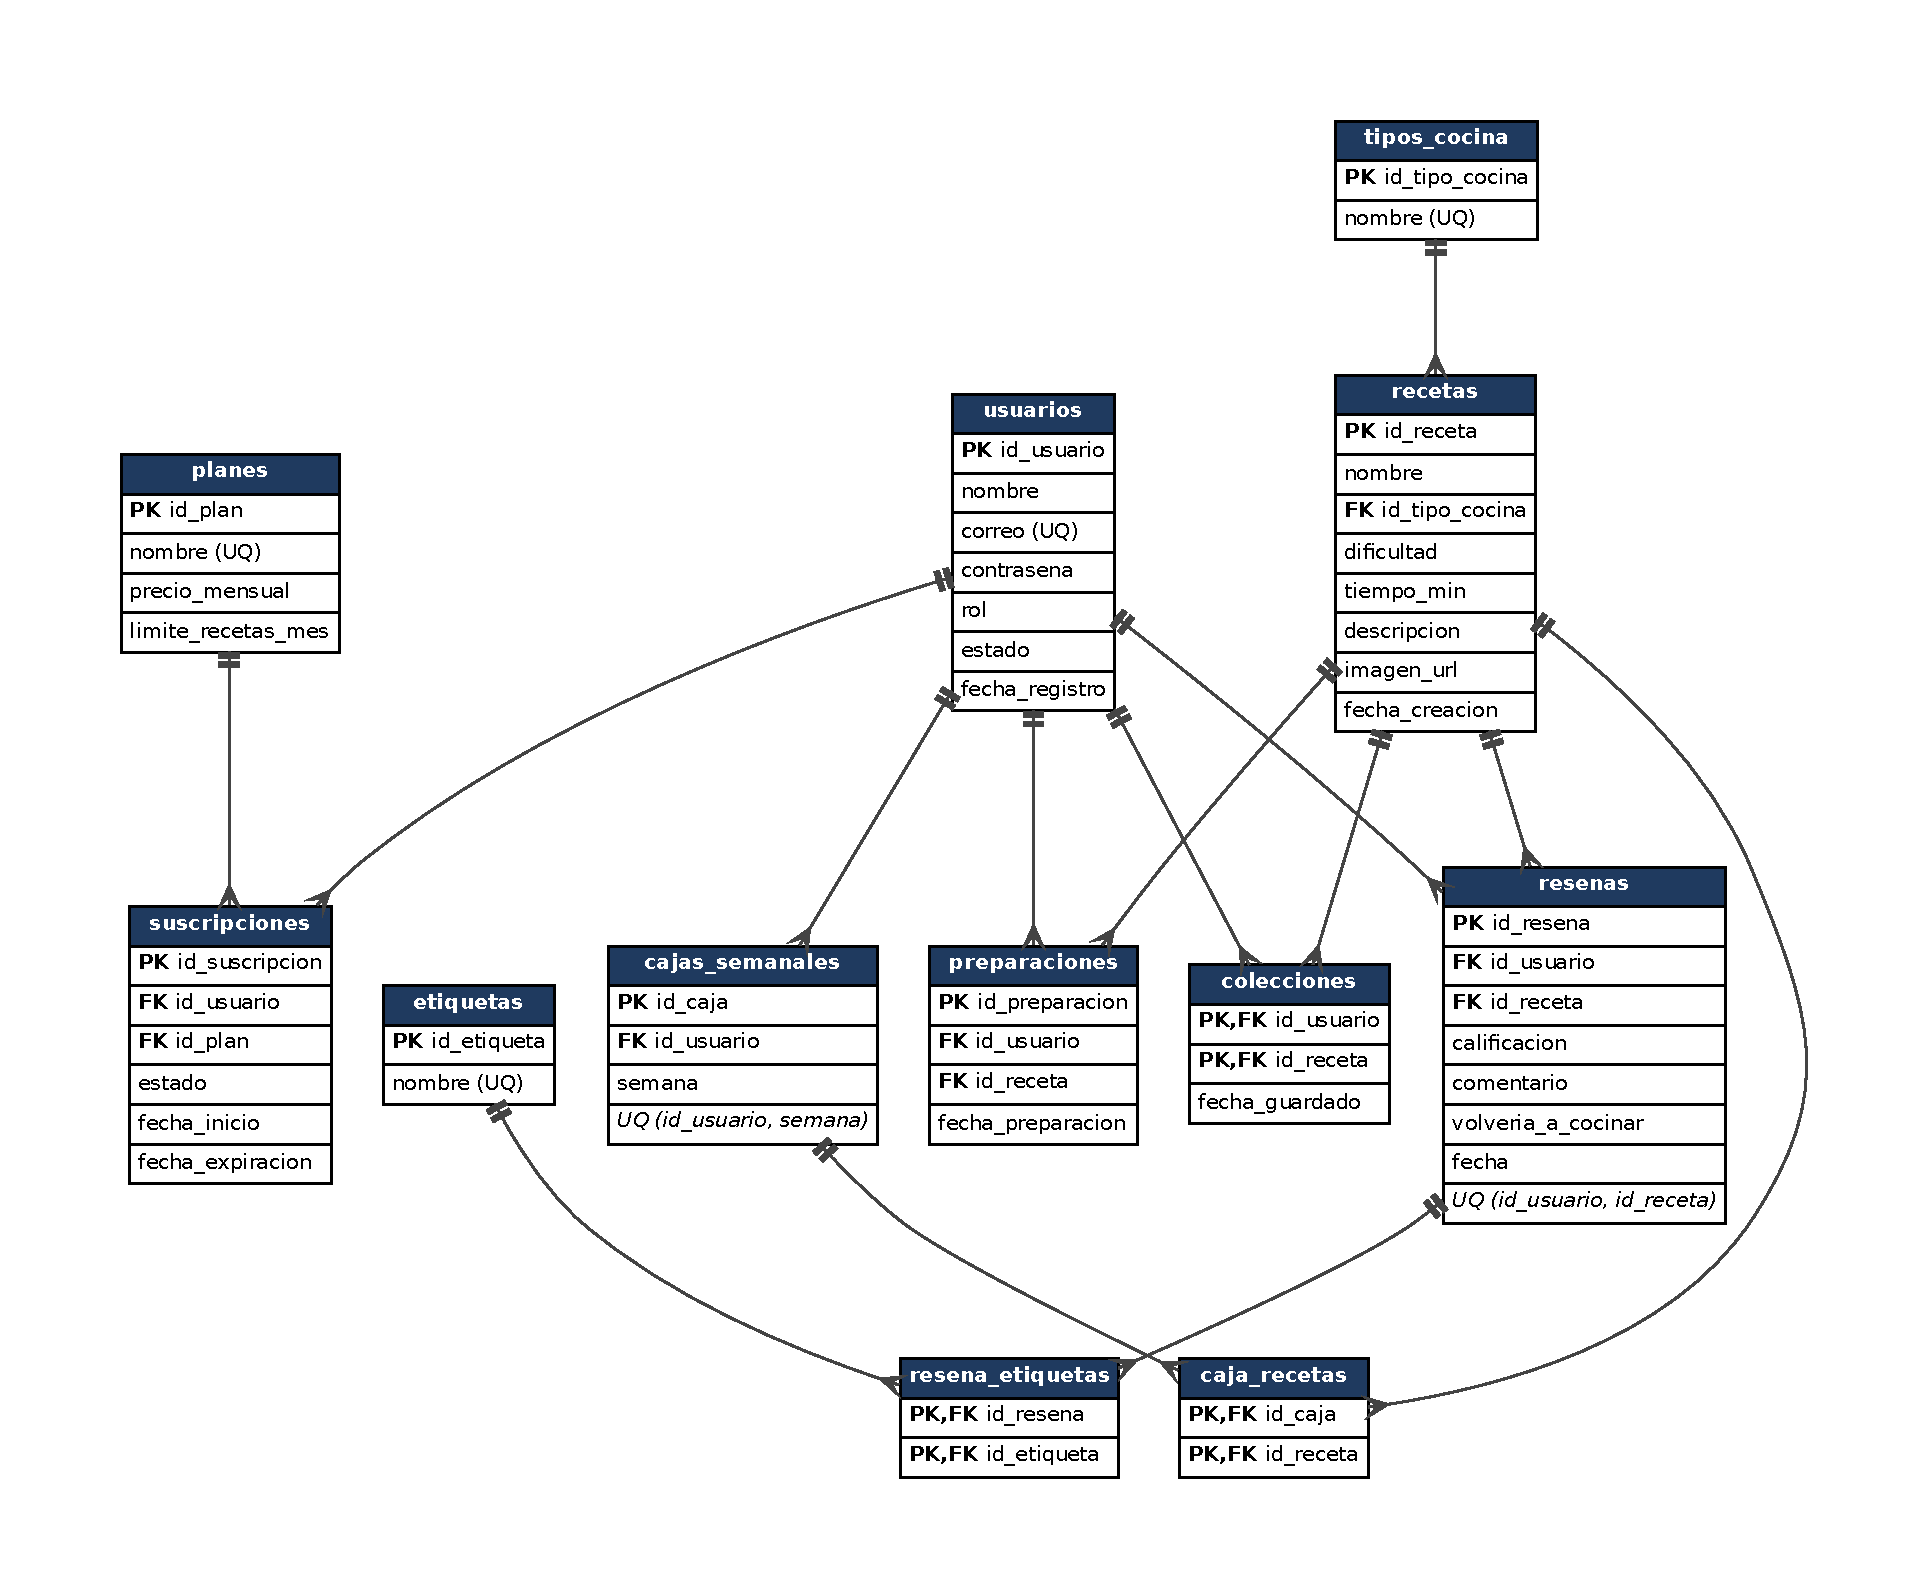
\includegraphics[width=0.82\textwidth]{er.pdf}
\caption{Diagrama entidad--relación de TasteBox. PK: clave primaria; FK: clave foránea; UQ: restricción de unicidad. En cada vínculo, el extremo con doble barra indica ``uno'' y la pata de gallo indica ``muchos''.}
\label{fig:er}
\end{figure*}

\subsection{Cardinalidades y reglas de integridad}
La Tabla~\ref{tab:card} resume las cardinalidades y la regla de borrado referencial elegida para cada vínculo. La política de borrado no es uniforme porque responde a la naturaleza de cada dependencia: los datos personales y de actividad de un usuario dependen de su cuenta y se eliminan con ella (\cd{CASCADE}), mientras que los catálogos referenciados (planes y tipos de cocina) se protegen con \cd{RESTRICT}, de modo que no pueda borrarse un plan o una cocina en uso. El efecto práctico se verifica en la API: eliminar un tipo de cocina con recetas asociadas responde 409.

\begin{table}[!t]
\caption{Cardinalidades y política de borrado referencial}
\label{tab:card}
\centering
\footnotesize
\renewcommand{\arraystretch}{1.15}
\begin{tabular}{@{}p{3.6cm}cp{2.2cm}@{}}
\toprule
\textbf{Vínculo (padre $\rightarrow$ hijo)} & \textbf{Card.} & \textbf{Al borrar el padre} \\
\midrule
Usuario $\rightarrow$ Suscripción & 1:N & CASCADE \\
Plan $\rightarrow$ Suscripción & 1:N & RESTRICT \\
Tipo de cocina $\rightarrow$ Receta & 1:N & RESTRICT \\
Usuario $\rightarrow$ Colección & 1:N & CASCADE \\
Receta $\rightarrow$ Colección & 1:N & CASCADE \\
Usuario $\rightarrow$ Preparación & 1:N & CASCADE \\
Receta $\rightarrow$ Preparación & 1:N & CASCADE \\
Usuario $\rightarrow$ Reseña & 1:N & CASCADE \\
Receta $\rightarrow$ Reseña & 1:N & CASCADE \\
Reseña $\rightarrow$ Reseña--Etiqueta & 1:N & CASCADE \\
Etiqueta $\rightarrow$ Reseña--Etiqueta & 1:N & CASCADE \\
Usuario $\rightarrow$ Caja semanal & 1:N & CASCADE \\
Caja $\rightarrow$ Caja--Receta & 1:N & CASCADE \\
Receta $\rightarrow$ Caja--Receta & 1:N & CASCADE \\
\bottomrule
\end{tabular}
\end{table}

Las cardinalidades N:M resultantes son Usuario--Receta (por guardado, por preparación y por reseña), Reseña--Etiqueta y Caja--Receta. Además de las claves, el esquema codifica reglas del caso como restricciones declarativas: el correo es único (HU-01); un usuario solo puede reseñar una vez cada receta, mediante \cd{UNIQUE(id_usuario, id_receta)} (HU-07); una caja es única por usuario y semana; y \cd{CHECK} limita la calificación a 1--5 y el tiempo de preparación a valores positivos.

Dos decisiones merecen justificación explícita. Primero, \cd{preparaciones} usa una clave sustituta y \emph{no} una clave compuesta, porque un usuario puede preparar la misma receta muchas veces y cada ocurrencia es un hecho distinto (alimenta la racha y los conteos mensuales); en cambio \cd{colecciones} sí usa clave compuesta porque guardar dos veces la misma receta no tiene sentido. Segundo, las columnas de dominio cerrado y pequeño (\cd{rol}, \cd{estado}, \cd{dificultad}) se definen como \cd{ENUM} en lugar de tablas de consulta: su conjunto de valores forma parte de la lógica de la aplicación y no lo administra el usuario, a diferencia de los tipos de cocina y las etiquetas. El costo asumido es que agregar un valor exige modificar el esquema.

\subsection{Proceso de normalización}
La normalización se aplicó partiendo de una relación universal que reúne los atributos de todas las historias de usuario. Se muestra de forma abreviada:

\vspace{2pt}
\noindent\footnotesize\texttt{R0(id\_usuario, nombre, correo, contrasena, rol,\\
\hspace*{1.5em}plan\_nombre, plan\_precio, plan\_limite, fecha\_inicio, fecha\_exp,\\
\hspace*{1.5em}id\_receta, nombre\_receta, tipo\_cocina, dificultad, tiempo,\\
\hspace*{1.5em}calificacion, comentario, \{etiquetas\}, fecha\_guardado,\\
\hspace*{1.5em}\{fechas\_preparacion\}, semana\_caja, \{recetas\_caja\})}
\normalsize
\vspace{2pt}

Esta relación presenta las tres anomalías clásicas. Hay anomalía de inserción, porque no puede registrarse una receta del catálogo mientras ningún usuario la haya reseñado o guardado (HU-15 exige lo contrario). Hay anomalía de actualización, porque cambiar el precio del plan Premium obligaría a modificar todas las filas de todos los suscriptores, y escribir ``Italiana'' de dos formas distintas rompería los filtros de HU-03. Y hay anomalía de borrado, porque eliminar la última reseña de una receta eliminaría también los datos de la receta. Los pasos siguientes eliminan cada causa.

\textbf{Primera forma normal (1FN).} R0 contiene atributos multivaluados (las etiquetas de una reseña, las fechas de preparación y las recetas de una caja). Cada uno se extrae a una relación donde cada celda guarda un solo valor: \cd{resena_etiquetas}, \cd{preparaciones} y \cd{caja_recetas}. Con ello todos los atributos son atómicos y cada relación tiene clave primaria.

\textbf{Segunda forma normal (2FN).} Se detectan dependencias parciales sobre claves compuestas. En la relación Reseña, con clave candidata (\cd{id_usuario}, \cd{id_receta}), el nombre y la dificultad de la receta dependen solo de \cd{id_receta}, y el correo solo de \cd{id_usuario}. Se separan las entidades \cd{usuarios} y \cd{recetas}, y las relaciones \cd{resenas}, \cd{colecciones} y \cd{preparaciones} conservan únicamente las claves foráneas y los atributos propios del hecho (calificación, comentario, fechas). Las relaciones asociativas \cd{colecciones}, \cd{resena_etiquetas} y \cd{caja_recetas} cumplen 2FN porque su único atributo no clave, cuando existe, depende de la clave completa.

\textbf{Tercera forma normal (3FN).} Quedan dependencias transitivas. En \cd{suscripciones}, \cd{id_plan} determina nombre, precio y límite, y \cd{id_suscripcion} solo determina esos valores a través de \cd{id_plan}; se extrae \cd{planes}. Del mismo modo, en \cd{recetas}, el nombre de la cocina depende de \cd{id_tipo_cocina} y no de la receta; se extrae \cd{tipos_cocina}. Esta decisión resuelve la anomalía de actualización descrita arriba: el precio de un plan o el nombre de una cocina se almacena una sola vez.

\textbf{Forma normal de Boyce--Codd (BCNF).} Se verificó que todo determinante sea superclave. La Tabla~\ref{tab:fd} lista las claves candidatas y las dependencias funcionales no triviales. En \cd{usuarios} existen dos determinantes, \cd{id_usuario} y \cd{correo}, y ambos son claves candidatas; lo mismo ocurre en \cd{resenas} con \cd{id_resena} y el par (\cd{id_usuario}, \cd{id_receta}). Como no hay un determinante que no sea clave, el esquema alcanza BCNF, que es más estricta que la 3FN pedida como mínimo.

\begin{table}[!t]
\caption{Claves candidatas y dependencias funcionales}
\label{tab:fd}
\centering
\footnotesize
\renewcommand{\arraystretch}{1.15}
\begin{tabular}{@{}p{1.9cm}p{2.5cm}p{3.2cm}@{}}
\toprule
\textbf{Relación} & \textbf{Claves candidatas} & \textbf{Dependencias no triviales} \\
\midrule
\cd{usuarios} & \cd{id_usuario}; \cd{correo} & \cd{id_usuario} $\rightarrow$ resto; \cd{correo} $\rightarrow$ resto \\
\cd{planes} & \cd{id_plan}; \cd{nombre} & \cd{id_plan} $\leftrightarrow$ \cd{nombre}; $\rightarrow$ precio, límite \\
\cd{suscripciones} & \cd{id_suscripcion} & $\rightarrow$ usuario, plan, estado, fechas \\
\cd{tipos_cocina} & \cd{id_tipo_cocina}; \cd{nombre} & \cd{id_tipo_cocina} $\leftrightarrow$ \cd{nombre} \\
\cd{recetas} & \cd{id_receta} & $\rightarrow$ nombre, cocina, dificultad, tiempo, \ldots \\
\cd{colecciones} & (\cd{id_usuario}, \cd{id_receta}) & $\rightarrow$ \cd{fecha_guardado} \\
\cd{preparaciones} & \cd{id_preparacion} & $\rightarrow$ usuario, receta, fecha \\
\cd{resenas} & \cd{id_resena}; (\cd{id_usuario}, \cd{id_receta}) & $\rightarrow$ calificación, comentario, volvería, fecha \\
\cd{resena_etiquetas} & (\cd{id_resena}, \cd{id_etiqueta}) & ninguna \\
\cd{cajas_semanales} & \cd{id_caja}; (\cd{id_usuario}, \cd{semana}) & $\rightarrow$ usuario, semana \\
\cd{caja_recetas} & (\cd{id_caja}, \cd{id_receta}) & ninguna \\
\bottomrule
\end{tabular}
\end{table}

\subsection{Desnormalización y limitaciones asumidas}
\textbf{No se aplicó ninguna desnormalización en las tablas.} La única tentación evidente era guardar en \cd{recetas} la calificación promedio y el número de reseñas para acelerar el catálogo. Se descartó porque duplicaría un dato derivable, exigiría actualizarlo en cada alta, edición o baja de reseña (con riesgo de inconsistencia si alguna ruta lo olvida) y no es necesario para cumplir RNF-01: el promedio se calcula con \cd{AVG()} y \cd{COUNT()} en la misma consulta del catálogo, con tiempos de respuesta de pocos milisegundos en las pruebas realizadas. Si el volumen creciera de forma que ese cálculo incumpliera el umbral de 3~s, la columna redundante sería la primera optimización a considerar, acompañada de un disparador o de una actualización transaccional.

Se asumen también tres limitaciones deliberadas de este corte. (i) \emph{La contraseña se almacena en texto plano}, como exige la definición del corte; esto incumple RNF-03 y se acepta únicamente en este entregable. La corrección prevista consiste en reemplazar la comparación directa por una función de derivación adaptativa como Argon2id o bcrypt con sal \cite{owasp,nist}, sin cambiar el esquema salvo la longitud de la columna. (ii) La regla ``una sola suscripción activa por usuario'' no se impone en la base de datos, porque MySQL no ofrece índices únicos parciales; se garantiza en la capa de servicios, que cancela la suscripción vigente y crea la nueva dentro de una transacción, conservando el historial. (iii) El borrado de una receta elimina en cascada sus preparaciones, lo que altera los hábitos históricos; en producción sería preferible un borrado lógico.

\section{Identificación y diseño de recursos REST}

\subsection{Criterios de diseño}
El diseño sigue el estilo REST propuesto por Fielding \cite{fielding} y la semántica de métodos y códigos de estado de HTTP \cite{rfc9110}. Se adoptaron cuatro criterios: (1) los recursos se nombran con sustantivos en plural y las acciones se expresan con el verbo HTTP, no con la URI; (2) \cd{GET} no modifica estado; \cd{PUT} reemplaza o actualiza de forma idempotente; \cd{POST} crea; \cd{DELETE} elimina; (3) cada resultado se comunica con un código de estado significativo (201 al crear, 204 al eliminar, 400, 401, 403, 404 y 409 para los distintos errores); y (4) la URI refleja la propiedad de los datos, de modo que una colección que pertenece a un usuario cuelga de ese usuario.

\subsection{Mapeo de entidades a recursos}
No existe una correspondencia uno a uno entre tablas y recursos, y esa asimetría es una decisión de diseño. La Tabla~\ref{tab:map} muestra cómo se resolvió cada entidad y por qué.

\begin{table*}[!t]
\caption{Mapeo de entidades del modelo de datos a recursos REST}
\label{tab:map}
\centering
\footnotesize
\renewcommand{\arraystretch}{1.2}
\begin{tabular}{@{}p{2.7cm}p{4.2cm}p{9.8cm}@{}}
\toprule
\textbf{Entidad} & \textbf{Recurso (URI)} & \textbf{Decisión de diseño} \\
\midrule
Usuario & \cd{/usuarios}, \cd{/usuarios/:id} & Recurso de primer nivel. El registro y el inicio de sesión se separan en \cd{/auth/*} porque no son operaciones CRUD sobre un usuario ya existente, sino procesos de acceso. \\
Receta & \cd{/recetas}, \cd{/recetas/:id} & Recurso de primer nivel con búsqueda y filtros como parámetros de consulta (\cd{q}, \cd{cocina}, \cd{dificultad}, \cd{pagina}), porque filtrar no crea un recurso nuevo. La respuesta incluye el promedio y el total de reseñas. \\
Reseña & \cd{/recetas/:id/resenas} (listar, crear) y \cd{/resenas/:id} (editar, borrar) & Anidada para crear y listar, porque una reseña no tiene sentido sin su receta y el padre queda explícito en la URI. Para editar y borrar se usa una URI plana, porque \cd{id_resena} ya identifica unívocamente el recurso y repetir la receta añadiría redundancia y un caso de error (receta que no corresponde). \\
Colección & \cd{/usuarios/:id/coleccion} y \cd{/usuarios/:id/coleccion/:idReceta} & Anidada bajo el usuario por propiedad. Es un recurso asociativo: no tiene identificador propio, se identifica por el par (usuario, receta); por eso se agrega con \cd{POST} (cuerpo \cd{id_receta}) y se quita con \cd{DELETE} sobre la receta. \\
Preparación & \cd{/usuarios/:id/preparaciones} & Anidada bajo el usuario. Solo admite alta y consulta: una preparación es un hecho histórico y no se edita. \\
Hábitos & \cd{/usuarios/:id/habitos} & \emph{Endpoint compuesto} de solo lectura. No corresponde a ninguna tabla: agrega preparaciones por mes, por cocina, racha y actividad reciente. \\
Suscripción y plan & \cd{/usuarios/:id/suscripcion}, \cd{/planes}, \cd{/suscripciones} & La suscripción vigente se trata como un recurso singular del usuario. El cambio a Premium se modela como \cd{PUT} que fija el plan (\cd{id_plan}) y no como una acción \cd{POST /premium}, porque lo que se modifica es el estado del recurso. \cd{/suscripciones} es la vista global del administrador y \cd{/planes} es un catálogo de lectura. \\
Caja semanal & \cd{/usuarios/:id/caja-semanal} & Anidada bajo el usuario y filtrable por \cd{semana}. Incluye en la respuesta las recetas de la caja (relación resuelta por \emph{incrustación}, no por referencias que obliguen a otra consulta). \\
Tipo de cocina, etiqueta & \cd{/tipos-cocina}, \cd{/etiquetas} & Catálogos de lectura pública y escritura restringida al administrador. \\
Panel & \cd{/admin/resumen} & Endpoint compuesto de solo lectura (RF-15) que reúne conteos de usuarios, recetas, preparaciones y suscripciones. \\
\bottomrule
\end{tabular}
\end{table*}

\subsection{Resolución de las relaciones entre recursos}
Se emplearon tres mecanismos, escogidos según el tipo de relación. El \textbf{anidamiento} se usa cuando el hijo no existe sin el padre o le pertenece (reseñas de una receta; colección, preparaciones, suscripción y caja de un usuario). Su ventaja es que la URI documenta la propiedad y permite aplicar la regla de autorización ``el propio usuario o un administrador'' una sola vez sobre \cd{/usuarios/:id/*}. Su límite es la profundidad: se evitó pasar de dos niveles, y por eso la edición de reseñas es plana.

Las \textbf{referencias por identificador} se usan cuando la relación es entre recursos independientes. Una receta referencia su tipo de cocina con \cd{id_tipo_cocina}, y para guardar una receta o marcarla como preparada el cuerpo lleva \cd{id_receta}. Referenciar en el cuerpo, y no en la URI, evita URIs como \cd{/usuarios/3/coleccion/7} para una operación de creación, donde el cliente aún no conoce un identificador de recurso propio. La API valida que la referencia exista y responde 404 o 400 según el caso, en lugar de dejar que la restricción de la base de datos produzca un error opaco.

Los \textbf{endpoints compuestos} se usan cuando el cliente necesita información que atraviesa varias tablas o que se calcula: los hábitos, el panel del administrador y el detalle de receta con calificación promedio. Reducen el número de solicitudes del cliente y mantienen la lógica de agregación en el servidor.

\subsection{Endpoints y trazabilidad con los requerimientos}
La API expone 37 operaciones sobre 22 rutas. La Tabla~\ref{tab:endpoints} las agrupa y las vincula con los requerimientos funcionales del corte 1; con ello se comprueba que cada RF tiene al menos un endpoint que lo implementa. Las operaciones que no figuran con un RF propio (catálogos auxiliares) existen para sostener los datos que otros RF requieren, como los tipos de cocina que se asignan a una receta.

\begin{table*}[!t]
\caption{Endpoints de la API y requerimientos funcionales que implementan}
\label{tab:endpoints}
\centering
\footnotesize
\renewcommand{\arraystretch}{1.12}
\begin{tabular}{@{}p{2.3cm}p{5.2cm}p{5.8cm}p{2.5cm}@{}}
\toprule
\textbf{Método} & \textbf{Ruta} & \textbf{Descripción} & \textbf{RF / acceso} \\
\midrule
POST & \cd{/auth/registro} & Registra un usuario (plan gratuito) & RF-01, público \\
POST & \cd{/auth/login} & Verifica credenciales y devuelve JWT & RF-02, público \\
GET & \cd{/recetas} & Catálogo con búsqueda, filtros y paginación & RF-03, RF-04 \\
GET & \cd{/recetas/:id} & Detalle de receta & RF-05 \\
POST, PUT, DEL. & \cd{/recetas}, \cd{/recetas/:id} & Alta, edición y baja de recetas & RF-16, RF-17, admin \\
POST & \cd{/usuarios/:id/coleccion} & Guarda una receta en la colección & RF-06 \\
GET, DEL. & \cd{/usuarios/:id/coleccion}, \cd{.../:idReceta} & Consulta y quita recetas guardadas & RF-06 \\
POST, GET & \cd{/usuarios/:id/preparaciones} & Marca receta preparada; lista preparaciones & RF-07 \\
POST, GET & \cd{/recetas/:id/resenas} & Crea y consulta reseñas de una receta & RF-08, RF-09 \\
PUT, DEL. & \cd{/resenas/:id} & Edita o elimina una reseña propia & RF-08 \\
GET & \cd{/usuarios/:id/habitos} & Indicadores de hábitos de cocina & RF-10 \\
GET & \cd{/usuarios/:id/suscripcion} & Plan vigente y uso del plan gratuito & RF-11 \\
PUT & \cd{/usuarios/:id/suscripcion} & Cambio de plan (a Premium) & RF-12 \\
GET, POST, DEL. & \cd{/usuarios/:id/caja-semanal} (y \cd{/:idCaja}) & Consulta, asigna y elimina la caja semanal & RF-13 \\
GET, PUT & \cd{/usuarios/:id} & Consulta y edición de perfil & RF-14 \\
GET & \cd{/admin/resumen} & Panel de resumen & RF-15, admin \\
GET & \cd{/suscripciones} & Suscripciones con búsqueda y filtros & RF-18, admin \\
GET, DEL. & \cd{/usuarios}, \cd{/usuarios/:id} & Lista, busca y elimina usuarios; PUT cambia rol y estado & RF-19, admin \\
CRUD & \cd{/tipos-cocina}, \cd{/etiquetas} & Catálogos auxiliares (lectura pública) & soporte, admin \\
GET & \cd{/planes} & Planes disponibles & soporte, público \\
\bottomrule
\end{tabular}
\end{table*}

\subsection{Autenticación, autorización y reglas de negocio}
El inicio de sesión devuelve un token JWT firmado \cite{rfc7519} que contiene el identificador y el rol del usuario, y que el cliente envía en el encabezado \texttt{Authorization: Bearer}. Se eligió un token sin estado en el servidor para no introducir una tabla de sesiones en este corte. Tres middlewares aplican las reglas de seguridad del corte 1: \cd{autenticar} (RNF-05) rechaza con 401 las solicitudes sin token válido; \cd{soloAdmin} (RNF-04) responde 403 a cuentas sin rol de administrador; y \cd{propioOAdmin} restringe los recursos \cd{/usuarios/:id/*} a su dueño o a un administrador. Así, un usuario que consulta la colección o los hábitos de otro recibe 403 y no los datos.

Las reglas de negocio explícitas del caso se implementan en la capa de servicios y se prueban en la colección: el plan gratuito permite hasta cinco recetas preparadas por mes (el valor es una decisión del equipo documentada en la Sección~XII y se almacena en \cd{planes}, no en el código); la caja semanal solo puede asignarse y consultarse para usuarios Premium y su semana debe iniciar en lunes; un usuario solo puede reseñar una vez cada receta; y solo el autor o un administrador puede modificar una reseña.

\subsection{Validación y formato de errores}
La validación de entrada se hace en un middleware previo al controlador, con reglas declarativas por recurso: campos obligatorios, tipo (cadena, entero, booleano, arreglo de enteros), longitudes, rangos (calificación de 1 a 5), enumeraciones (dificultad, rol, estado), formato de correo y de fecha. Las actualizaciones (\cd{PUT}) aceptan cualquier subconjunto de campos, pero exigen al menos uno. Todos los errores comparten una estructura \texttt{\{ error, detalles \}}, donde \cd{detalles} lista el campo y el mensaje de cada violación, de modo que el cliente pueda mostrar el problema junto al campo correspondiente (RNF-08).

\section{Arquitectura de la API}

\subsection{Organización por capas}
El proyecto se organiza en capas con una dependencia estrictamente descendente: cada capa conoce solo a la inmediatamente inferior (Fig.~\ref{fig:capas}). La separación persigue que un cambio en una preocupación (por ejemplo, la regla del límite mensual) afecte a un único archivo, y que cada capa pueda probarse de forma aislada.

\begin{figure}[!t]
\centering
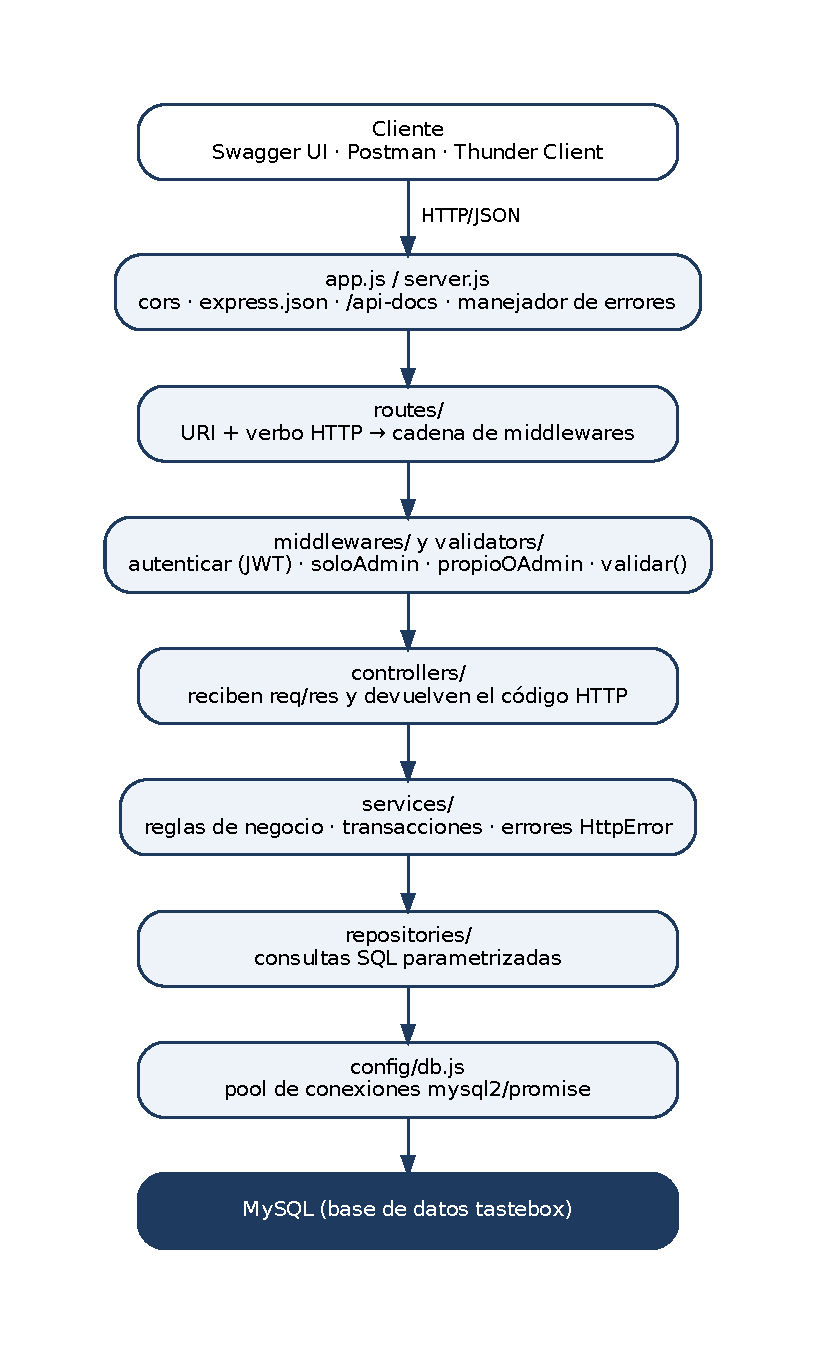
\includegraphics[width=0.92\columnwidth]{arquitectura.pdf}
\caption{Arquitectura por capas de la API.}
\label{fig:capas}
\end{figure}

La Tabla~\ref{tab:capas} detalla la responsabilidad de cada capa. La regla que ordena el diseño es que las capas superiores traducen HTTP y las inferiores no saben que HTTP existe: los repositorios devuelven filas, los servicios lanzan errores de dominio (\cd{HttpError}) y solo el manejador central de errores los convierte en respuestas.

\begin{table}[!t]
\caption{Responsabilidades por capa}
\label{tab:capas}
\centering
\footnotesize
\renewcommand{\arraystretch}{1.15}
\begin{tabular}{@{}p{1.7cm}p{5.7cm}@{}}
\toprule
\textbf{Capa} & \textbf{Responsabilidad} \\
\midrule
\cd{routes/} & Asocia ruta y verbo con la cadena de middlewares y el controlador; no contiene lógica. \\
\cd{middlewares/}, \cd{validators/} & Autenticación y autorización por rol; validación del cuerpo y de los parámetros de ruta; manejo central de errores. \\
\cd{controllers/} & Extraen datos de la solicitud, invocan al servicio y fijan el código de estado (201, 204, 200). \\
\cd{services/} & Reglas de negocio (límites del plan, Premium, una reseña por receta), orquestación de varios repositorios y transacciones. \\
\cd{repositories/} & Única capa que escribe SQL; consultas parametrizadas, sin lógica de negocio. \\
\cd{config/} & Pool de conexiones a MySQL. \\
\bottomrule
\end{tabular}
\end{table}

\subsection{Conexión a MySQL}
El acceso a datos usa el controlador \cd{mysql2} en su variante basada en promesas. En lugar de abrir una conexión por solicitud, se crea un \emph{pool} con un máximo de diez conexiones reutilizables al iniciar la aplicación; las credenciales se leen de variables de entorno (\cd{.env}, excluido del repositorio). Todas las consultas utilizan marcadores de posición (\cd{?}), de modo que los valores viajan separados del texto SQL, lo que previene la inyección SQL. Las fechas se devuelven como texto (\cd{dateStrings}) para evitar desplazamientos por zona horaria.

Las operaciones que modifican varias tablas se ejecutan en una \emph{transacción} gestionada por una utilidad que obtiene una conexión del pool, confirma si todo termina bien y revierte ante cualquier error. Se usa en el registro (usuario y suscripción gratuita), en el cambio de plan (cancelar la suscripción vigente y crear la nueva), en la creación de reseñas con sus etiquetas y en la asignación de cajas con sus recetas; en todos los casos, un fallo a mitad de camino no deja datos a medias.

Los errores de la base de datos se traducen a códigos HTTP en el manejador central: una violación de unicidad produce 409, una referencia inexistente 400 y el borrado de un registro en uso 409. Los detalles internos de un error inesperado se registran en el servidor y no se envían al cliente (500 genérico).

\subsection{Estructura del proyecto}
\begin{footnotesize}
\begin{verbatim}
tastebox-api/
  database/schema.sql   esquema y datos
  src/
    server.js, app.js   arranque
    config/db.js        pool MySQL
    routes/             rutas por recurso
    middlewares/        auth, errores
    validators/         validacion de entrada
    controllers/        uno por recurso
    services/           reglas de negocio
    repositories/       consultas SQL
    docs/openapi.js     especificacion OpenAPI
    utils/              errores, transacciones
  scripts/              init-db, openapi, postman
  postman/              coleccion de pruebas
\end{verbatim}
\end{footnotesize}

\subsection{Documentación y pruebas}
La especificación OpenAPI 3.0 se mantiene en un único módulo que describe cada operación (parámetros, cuerpo, respuestas de éxito y de error con ejemplos \cite{openapi}) y se publica con Swagger UI en la ruta \cd{/api-docs}, donde cada endpoint puede ejecutarse de forma interactiva tras autorizar el token. La colección de pruebas contiene 99 solicitudes, con al menos un caso de éxito y uno de error por endpoint, y 248 aserciones sobre el código de estado y la forma de la respuesta. Se ejecuta de forma encadenada: el inicio de sesión guarda el token en variables de la colección y las altas guardan los identificadores que usan las solicitudes siguientes. En la última ejecución completa, las 248 aserciones pasaron y la colección puede repetirse sin reiniciar la base de datos, porque la limpieza final elimina los datos que ella misma crea.
